\documentclass[aspectratio=169]{beamer}

% Custom theme and packages
\usepackage{beamertheme-custom}
% Custom symbols and commands
\usepackage{symbols-custom}
\usepackage{ 
    enumitem,
    booktabs}


\usepackage{ 
    tikz,
    tikz-qtree,
    xcolor}
    
\usepackage{graphicx}
\graphicspath{{figures/}}
\usetikzlibrary{trees}
\usetikzlibrary{tikzmark}

\title{Multinomial Processing Trees}
\author{Joachim Vandekerckhove}
\date{Spring 2025}

\tikzset{% set up for transitions using tikz with beamer overlays
  invisible/.style={color=black!75!white},
  color on/.style={alt=#1{}{invisible}},
  alt/.code args={<#1>#2#3}{%
    \alt<#1>{\pgfkeysalso{#2}}{\pgfkeysalso{#3}} % \pgfkeysalso doesn't change the path
  },
}


\setlist[enumerate]{label=\bf\alph*)}


% Font
\usefonttheme[onlymath]{serif}

% Colors
\definecolor{darkgreen}{rgb}  {0.10, 0.50, 0.10}
\definecolor{red}{rgb}{1,0,0}

\begin{document}

\maketitle

\begin{frame}[fragile]{One-High-Threshold Model}

The one-high-threshold model with parameters $\rho$ (probability of remembering) and $\gamma$ (probability of guessing ``old'')\pause

The tree representation shows the ``flow'' of the process
\null\hspace{-01.5cm}
\begin{tabular}{ll}
  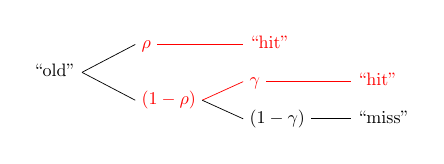
\begin{tikzpicture}[scale=0.65]
\tikzset{grow'=right}
\tikzset{execute at begin node=\strut}
\tikzset{every tree node/.style={anchor=base west}}
\tikzset{level 1/.style={level distance=60pt}}
\tikzset{level 2/.style={level distance=60pt}}
\tikzset{level 3+/.style={level distance=60pt}}
\Tree [.``old'' 	[.\node[color=red,color on=<4->]{$\rho$};\edge[draw=red,color on=<4->]; \node[color=red,color on=<4->]{``hit''}; ]
              		[.\node[color=red,color on=<5->]{$\left(1-\rho\right)$}; \edge[draw=red,color on=<5->];	[.\node[color=red,color on=<5->]{$\gamma$}; \edge[draw=red,color on=<5->]; \node[color=red,color on=<5->]{``hit''};  ]
						[.$\left(1-\gamma\right)$ ``miss'' ]
 ] ] 
\end{tikzpicture}
&
 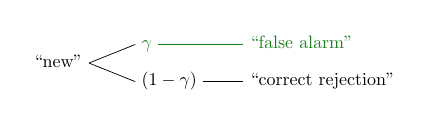
\begin{tikzpicture}[scale=0.65]
\tikzset{grow'=right}
\tikzset{execute at begin node=\strut}
\tikzset{every tree node/.style={anchor=base west}}
\tikzset{level 1/.style={level distance=60pt}}
\tikzset{level 2/.style={level distance=60pt}}
\tikzset{level 3+/.style={level distance=60pt}}
\Tree [.``new''		 [.\node[color=darkgreen,color on=<6->]{$\gamma$}; \edge[draw=darkgreen,color on=<6->]; \node[color=darkgreen,color on=<6->]{``false alarm''};]
              			[.$\left(1-\gamma\right)$ {``correct rejection''} ]
 ] ] 
\end{tikzpicture}
\end{tabular}\pause

The parameters $\rho$ and $\gamma$ together determine the hit rate $\theta^\mathrm{h}$ and false alarm rate $\theta^\mathrm{f}$
\begin{eqnarray}
 \theta^\mathrm{h} &=& {\color<4->{red}\rho} + {\color<5->{red}\left(1-\rho\right)\gamma} \nonumber\\
 \theta^\mathrm{f} &=& {\color<6->{darkgreen}\gamma} \nonumber
\end{eqnarray}

\end{frame}


\begin{frame}[fragile]{Weapon Priming Task}
Effect of stereotypes on the identification of objects in a weapon-identification task\pause

Participants presented with target images that they had to identify as a tool or a weapon\pause

On each trial, the target image was preceded by one of three primes: an image of a white face, black face, or a neutral outline\pause

Half the 82 participants had 500ms to respond, and the other half had 1000ms\pause

We consider only the white and black face primes, and how people make decisons about the tool and gun  targets in relation to the stereotype congruency and incongruency
\end{frame}

\begin{frame}[fragile]{Rivers et al.\ (2017) Data}
There were 1440 trials for each of the possibilities: white tool, white weapon, black tool, black weapon
conditions $\times$ two timing conditions

\begin{center}
\begin{tabular}{ccc}
\toprule
500ms & White & Black \\
\hline
 Tool & 885 (61\%) & 766 (53\%)\\
 Weapon & 967 (67\%) & 1074 (75\%) \\
\bottomrule
\end{tabular}
\end{center}

\begin{center}
\begin{tabular}{ccc}
\toprule
1000ms & White & Black \\
\hline
 Tool & 1280 (89\%) & 1229 (85\%)\\
 Weapon & 1281 (89\%) & 1288 (89\%) \\
\bottomrule
\end{tabular}
\end{center}

\end{frame}

\begin{frame}[fragile]{Weapon Priming MPT Model}
The ``Stroop'' model has sequential automatic, control, and guessing processes, controlled by three parameters
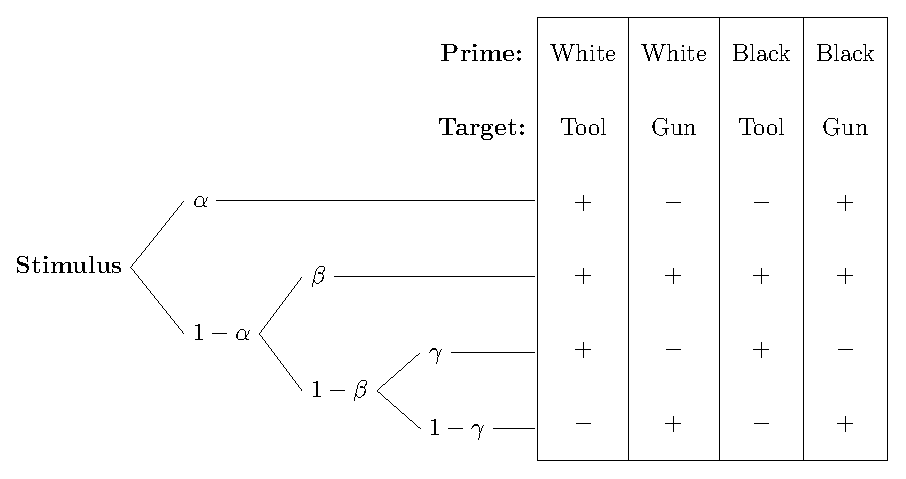
\includegraphics[width = 0.9\textwidth]{figures/weaponPriming.eps}
\end{frame}

\begin{frame}[fragile]{Weapon Priming MPT Model}
\begin{itemize}
\item The model involves three parameters, one for each process:
\begin{itemize}
\item[--] a probability $\alpha$ of an automatic process that answers ``tool'' for a white face prime and ``gun'' for a black face prime
\item[--] a probability $\beta$ of a control process that generates the correct answer
\item[--] a probability $\gamma$ of guessing ``tool''
\end{itemize}
\end{itemize}
\begin{center}
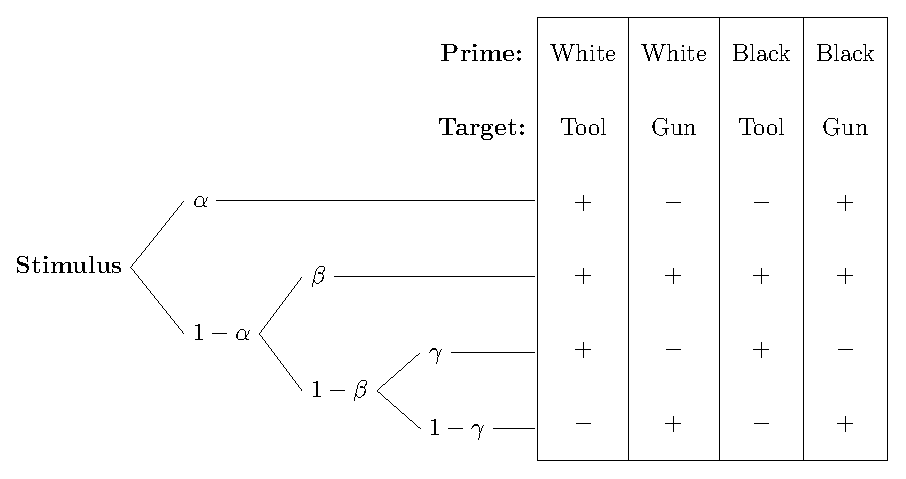
\includegraphics[width = 0.6\textwidth]{figures/weaponPriming.eps}
\end{center}
\end{frame}

\begin{frame}[fragile]{Weapon Priming MPT Model}
\vspace{-2em}
\begin{eqnarray}\small
\theta^{wt} &=& \alpha + \left(1-\alpha\right)\beta + \left(1-\alpha\right)\left(1-\beta\right)\gamma \nonumber\\
\theta^{bt} &=& \left(1-\alpha\right)\beta + \left(1-\alpha\right)\left(1-\beta\right)\gamma \nonumber\\
\theta^{wg} &=& \left(1-\alpha\right)\beta + \left(1-\alpha\right)\left(1-\beta\right)\left(1-\gamma\right) \nonumber\\
\theta^{bg} &=& \alpha + \left(1-\alpha\right)\beta + \left(1-\alpha\right)\left(1-\beta\right)\left(1-\gamma\right) \nonumber
\end{eqnarray}
\begin{center}
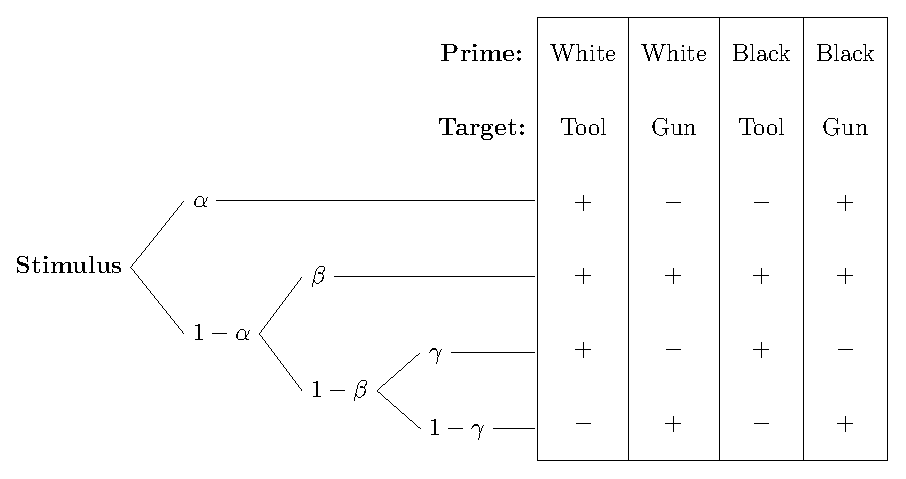
\includegraphics[width = 0.6\textwidth]{figures/weaponPriming.eps}
\end{center}
\end{frame}

\begin{frame}[fragile]{Weapon Priming MPT Model}
\begin{itemize}
\item For data that have $k^{\mathrm{wt}}$, $k^{\mathrm{bt}}$, $k^{\mathrm{wg}}$ and $k^{\mathrm{wg}}$ correct responses out of $n$ total trials, the model assumes that
\begin{eqnarray}
 k^{\mathrm{wt}} &\sim& \operatorname{binomial}\bigl(\theta^{\mathrm{wt}}, n\bigr) \nonumber\\
 k^{\mathrm{bt}} &\sim& \operatorname{binomial}\bigl(\theta^{\mathrm{bt}},  n\bigr) \nonumber\\
  k^{\mathrm{wg}} &\sim& \operatorname{binomial}\bigl(\theta^{\mathrm{wg}}, n\bigr) \nonumber\\
 k^{\mathrm{bg}} &\sim& \operatorname{binomial}\bigl(\theta^{\mathrm{bg}},  n\bigr) \nonumber
\end{eqnarray}
\item The model also assumes all automatic and control rates are equally likely,  and that guessing ``tool'' will happen around half the time: 
\begin{eqnarray}
\alpha &\sim& \operatorname{uniform}\bigl(0, 1\bigr) \nonumber\\
\beta &\sim&\operatorname{uniform}\bigl(0, 1\bigr) \nonumber\\
\gamma &\sim&\operatorname{beta}\bigl(3, 3\bigr) \nonumber
\end{eqnarray}
\end{itemize}
\vspace{1em}
\end{frame}


\begin{frame}[fragile]{Key Points}
\begin{itemize}
\item  The weapon-priming model is an example of an MPT model for addressing a social psychology phenomenon
\item Makes inferences about underlying executive control processes
\item The analysis of different deadline conditions in the experiment showed different use of automatic versus control processes
\end{itemize}
\vspace{8em}
\end{frame}


\end{document}
